\subsection{Polarisation}
Die Winkel mit den zugehörigen Intensitäten sind in Tabelle \ref{tab:Polarisation} aufgetragen. Die Funktion
\begin{align*}
	I_\text{fit} = I_0\sin^2\left(\omega\varphi + \varphi_0\right)
\end{align*}
wird an die Messwerte gefittet. Dabei ergeben sich die Parameter
\begin{align}
	I_0 &= \SI{94+-1e-6}{\micro\ampere}
 \\
	\omega &= \SI{1.013+-0.006}{}
 \\
	\varphi_0 &= \SI{0.44+-0.02}{}
 \ .
\end{align}
Die Messwerte und die gefittete Funktion sind in Abbildung \ref{fig:fitPol} zu sehen. Die Maxima befinden sich bei \SI{0.3\pi}{}
- bzw. $1.3\pi$, d.h. der Laser war in diese Richtung polarisiert.
\begin{figure}[h!]
	\centering
	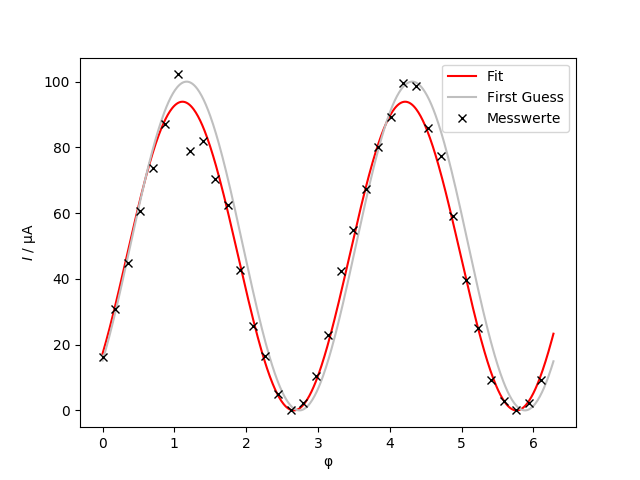
\includegraphics[width=.7\textwidth]{Fit_Polarisation.png}
	\caption{Fit zur Bestimmung der Polarisationsrichtung}
	\label{fig:fitPol}
\end{figure}
\begin{table}
    \centering
    \caption{Intensität in Abhängigkeit des Winkels des Polarisators}
    \label{tab:Polarisation}
    \sisetup{parse-numbers=false}
    \begin{tabular}{
	S[table-format=1.2]
	S[table-format=3.0]
	}
	\toprule
	{$\varphi$}		& {$I \ \mathrm{in} \ \si{\micro\ampere}$}		\\ 
	\midrule
    2.6 & 0.2   \\
2.8 & 2.4   \\
3.0 & 10.6  \\
3.1 & 23.0  \\
3.3 & 42.4  \\
3.5 & 54.8  \\
3.7 & 67.4  \\
3.8 & 80.2  \\
4.0 & 89.3  \\
4.2 & 99.5  \\
4.4 & 98.6  \\
4.5 & 85.8  \\
4.7 & 77.5  \\
4.9 & 59.0  \\
5.1 & 39.7  \\
5.2 & 25.2  \\
5.4 & 9.3   \\
5.6 & 3.0   \\
5.8 & 0.1   \\
5.9 & 2.1   \\
6.1 & 9.1   \\
0.0 & 16.2  \\
0.2 & 30.7  \\
0.3 & 44.9  \\
0.5 & 60.5  \\
0.7 & 73.6  \\
0.9 & 87.1  \\
1.0 & 102.2 \\
1.2 & 78.8  \\
1.4 & 81.9  \\
1.6 & 70.3  \\
1.7 & 62.5  \\
1.9 & 42.7  \\
2.1 & 25.7  \\
2.3 & 16.5  \\
2.4 & 5.0   \\

    \bottomrule
    \end{tabular}
    \end{table}
